% Change the following title and label as desired.
\section{Design and Implementation}
\label{sec:designandimplementation}

\subsection{System Description}
\label{sec:systemdescription}

At this stage, the autonomous wheelchair is developed to follow humans using the YOLOv11-based detection algorithm. The system is designed with the primary goal of enhancing the mobility of users who need assistance in moving. The system consists of hardware and software components, integrated to achieve this goal.

\vspace{5pt}
\subsubsection{System Components}
\label{subsubsec:systemcomponents}

The system consists of:

\begin{itemize}
    \item \textbf{VS Code}: Used as a development environment to run YOLOv11-related code and other analyses.
    \item \textbf{Arduino IDE}: Used to develop and upload code to the ESP32 that controls the motors and sensors.
    \item \textbf{Laptop}: Serves as the main data processing center for more complex tasks and software development.
    \item \textbf{Camera (OV5640 5MP)}: Captures real-time images of the environment and detects targets (humans) using YOLOv11.
    \item \textbf{ESP32 Devkit V1}: Acts as the main controller that manages data from the camera and controls the wheelchair's movement.
    \item \textbf{2 Motor Controllers}: Control the DC motors that drive the wheelchair.
    \item \textbf{2 DC-DC Voltage Regulators}: Regulate the voltage for electronic components to remain stable.
    \item \textbf{2 DC Motors}: Drive the wheelchair, controlled through motor drivers that receive signals from the microcontroller.
    \item \textbf{24V Battery}: Serves as the main power source for the entire system, including the microcontroller, motors, and other devices.
\end{itemize}

\vspace{5pt}
\subsubsection{System Architecture}
\label{subsubsec:systemarchitecture}

The system architecture is designed so that the camera continuously captures images, then sends the data to the ESP32 microcontroller for processing. YOLOv11 is used to detect humans and provide coordinate information of the target's position. This information is then used by the microcontroller to control the motors and direct the wheelchair to dynamically follow the target's movements.

\subsection{Hardware}
\label{subsec:hardware}

The hardware design involves the integration of several components mentioned earlier. The camera is mounted at the front of the wheelchair to obtain an optimal view of the target. The ESP32 microcontroller is placed at the bottom of the wheelchair along with the motor drivers and battery to maintain balance.

\begin{itemize}
    \item \textbf{Control Unit}: A control unit such as a computer or laptop is used as the main processing center to run YOLOv11 and MediaPipe, analyze detection results, and generate decisions in the form of instruction codes.
    \item \textbf{OV5640 Camera}: This camera is connected to the ESP32 to capture frames using a 5MP sensor.
    \item \textbf{ESP32}: This microcontroller receives data from the camera and then runs the algorithm to be processed on the computer, then sends control signals to the motor driver.
    \item \textbf{L298N Motor Driver}: This driver is used to control the speed and direction of the DC motors that drive the wheelchair.
\end{itemize}

\vspace{5pt}
\subsubsection{Camera}
\label{subsubsec:camera}

The camera used in this system is the OV5640, a CMOS (Complementary Metal-Oxide-Semiconductor) camera sensor with a resolution of 5 megapixels (MP). This sensor can capture images up to a maximum resolution of 2592x1944 pixels, providing highly detailed image results. The sensor supports real-time image and video capture, with a frame rate of up to 30 frames per second (fps) at 1080p resolution, making it ideal for applications requiring direct image processing.

In addition to its high resolution, the OV5640 is also equipped with various advanced features for automatic image processing. According to the datasheet, features such as auto white balance, auto exposure, and auto focus allow this camera to automatically adapt to changes in lighting conditions and distance, thus consistently producing high-quality images in various situations. The OV5640 also supports face detection and image scaling features, which are very useful for quickly and accurately detecting objects or human targets.

\vspace{5pt}
\subsubsection{Control Unit}
\label{subsubsec:controlunit}

The control unit in this system acts as the main data processor during testing, with specifications designed to handle high computational loads and suitable for real-time data processing.

One important aspect of the control unit in this project is the support for fast and stable WiFi communication between devices. The system relies on video data sent by the OV5640 camera through the ESP32 to the laptop for processing, and this process must occur without interruption. The provided WiFi connectivity also allows real-time data transmission with minimal latency, which is crucial for quick target detection.

The ability to maintain stable WiFi connections at greater distances from the router is also important for testing in large areas. Handling multiple devices connected simultaneously allows efficient communication between ESP32 units without performance degradation. This technology is essential to ensure that the system can continuously process video data sent by the camera and provide instructions with a quick response.

The image data obtained using the OV5640 camera will be processed through a series of image data processing steps using a pre-trained detection model. This model is trained using the YOLOv11 architecture. The model used is named Best.pt, which is the result of training to detect the Human class.

To implement the system properly, several libraries need to be installed first. These libraries include OpenCV for image processing and Ultralytics for YOLO.

\begin{lstlisting}
  pip install opencv-python
  pip install Ultralytics
  ...etc
\end{lstlisting}

\vspace{5pt}
\subsubsection{ESP32}
\label{subsubsec:ESP32}

The ESP32 will receive directional data from the human detection classification results in the form of character letters such as A, B, C, D, or E. Based on previous research, the process of receiving string data by the ESP32 from connected devices is crucial for the smooth operation of the system.

Once the data is received and stored, the string is extracted into information about direction and speed. This extraction stage is crucial to convert the string into a format that can be used by the program to control the wheelchair motors. The extracted data is then displayed to ensure that the received direction and speed match the expected values. With the direction and speed information ready, the ESP32 can send instructions to the wheelchair motors to move according to the received data. This process will continue as long as the device remains connected and data continues to flow.

To provide a clearer understanding of the instructions received from the human detection classification results, the following table presents the instruction codes used in this program:

\begin{table}[H]
\centering
\caption{Instruction Codes from Classification Results}
\begin{tabular}{|c|c|}
\hline
\textbf{Pose Classification} & \textbf{Instruction Code} \\
\hline
Left & A \\
\hline
Forward & B \\
\hline
Stop & C \\
\hline
Backward & D \\
\hline
Right & E \\
\hline
\end{tabular}
\end{table}

These instruction codes are used to direct the wheelchair motors according to the detections made by the YOLOv11 classification model. This program ensures that the ESP32 functions effectively as a server receiving data from the NUC and using it to control the wheelchair motors. With the steps described, this program is designed to run continuously without interruption, waiting for and processing data sent by connected devices.

\vspace{5pt}
\subsubsection{L298N Motor Driver}
\label{subsubsec:drivermotor}

The motor driver used in this system is the L298N, which plays a crucial role in controlling the DC motors of the wheelchair. This driver acts as an intermediary between the microcontroller and the motors, receiving control signals from the ESP32 and transmitting them to the motors. The use of the L298N driver allows digital signals to be converted into signals that can be accepted by the motors, enabling the motors to operate according to the given instructions.

The L298N driver can control two DC motors simultaneously with features for adjusting the speed and direction of motor rotation. This driver works on the principle of an H-Bridge circuit, which allows the direction of current to be changed to control the motor's forward or reverse rotation. Additionally, the L298N is equipped with speed control features through Pulse Width Modulation (PWM) techniques, providing more accurate control over motor speed. With these features, the wheelchair can move forward, backward, turn, or stop according to the received instructions.

\vspace{5pt}
\subsubsection{System Schematic}
\label{subsubsec:systemschematic}

From the research conducted, a control system for the wheelchair motors has been designed with the schematic shown in Figure \ref{fig:Wheelchair Motor Control Schematic}. The ESP32 will be connected to two H-Bridge Motor Drivers and a DC-DC Converter. Each H-Bridge Motor Driver is directly connected to the left and right wheel motors to effectively drive the wheelchair wheels. In this schematic, the ESP32 functions as the brain of the system, sending control signals to the motor drivers based on data received via WiFi. \cite{ekatama2024perancangan}

Thus, this program ensures that the ESP32 can function effectively as the wheelchair motor controller. Each step in the flowchart is designed to ensure that the system can operate efficiently and respond to commands received via the WiFi network. This system is designed to operate in real-time, providing quick responses to command changes and accurately controlling the wheelchair based on the received data.

The schematic shown provides a clear overview of the workflow and hardware connections used in this control system. With detailed explanations, every aspect of this system can be well understood, ensuring proper implementation and efficient operation of the autonomously controlled wheelchair. \cite{ekatama2024perancangan}

\begin{figure}[H]
  \centering

  % Replace with the image file name and size to be used
  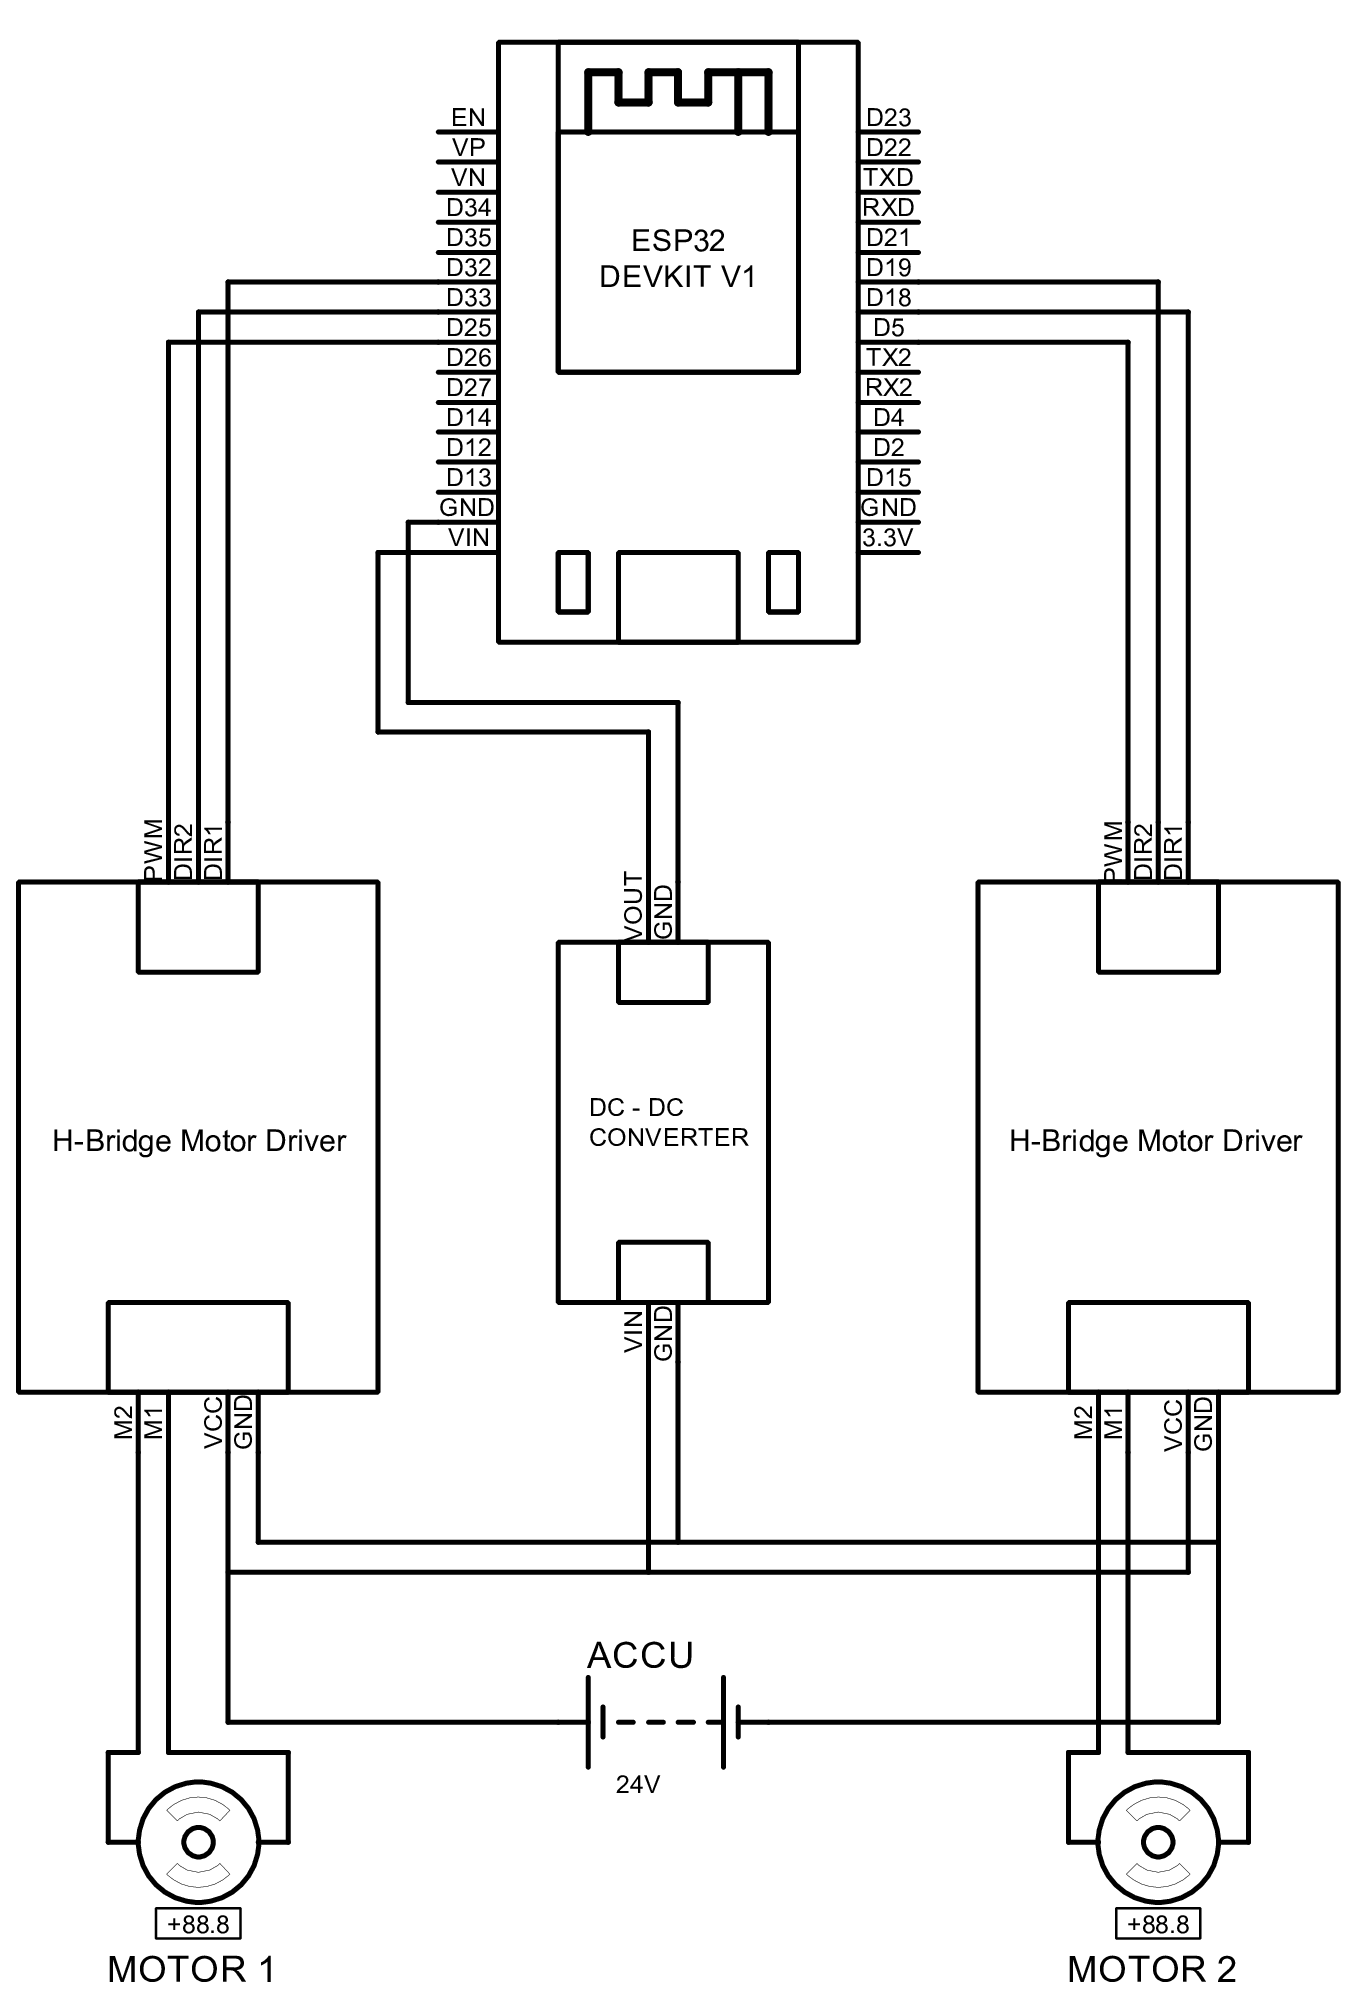
\includegraphics[scale=0.2]{gambar/Schematics.png}

  % Replace with the desired image caption
  \caption{Wheelchair Motor Control Schematic}
  \label{fig:Wheelchair Motor Control Schematic}
\end{figure}

\subsection{Software}
\label{subsec:software}

The software used in this system consists of several modules, including:

\begin{itemize}
    \item \textbf{YOLOv11 Detection Algorithm}: YOLOv11 is used to detect humans in images captured by the camera. This model is trained to recognize the shape and position of humans so that the wheelchair can accurately follow the target.
    \item \textbf{MediaPipe Pose Estimation}: MediaPipe is used to detect human body landmarks after the object is locked. This framework is chosen for its ability to detect keypoints on the human body with high accuracy, even in varying lighting conditions.
    \item \textbf{Data Communication}: The system uses the MQTT protocol to transmit data between the ESP32 connected to the camera and the main control unit.
    \item \textbf{Motor Control}: The motor control module is implemented on the ESP32 to adjust the direction and speed of the motors based on the detected target position.
\end{itemize}

\vspace{5pt}
\subsubsection{Image Dataset}
\label{subsubsec:imagedataset}

The image dataset used in this research consists of a collection of images taken using the OV5640 camera. The detected object in these images is a human, which serves as the target for the wheelchair to follow. The dataset includes various human poses and positions, as well as different lighting conditions, to optimally train the YOLOv11 model to recognize the target in various situations. These images are obtained from each video frame taken using the camera connected to the computer. The detection process is performed in real-time to ensure the system can continuously identify the target.

\vspace{5pt}
\subsubsection{Labeling}
\label{subsubsec:labeling}

The obtained image dataset then undergoes a labeling and augmentation process using tools like Roboflow, which provide various features to facilitate this process. The labeling process involves importing the dataset, labeling each image, and augmenting the data. Labeling is done to ensure that each object in the image is correctly recognized, especially the humans who are the target. The class naming must be consistent with the objects to be detected to ensure the YOLOv11 model can be properly trained.

Additionally, Roboflow provides dataset preprocessing features that help standardize the image format, such as resizing all images to a uniform size. This step is important to maintain dataset consistency before training the model. Available features include Auto-Orient, Resize, Grayscale, Auto Adjust Contrast, Isolate Objects, Static Crop, Tile, Modify Classes, and Filter Null. This preprocessing ensures that the data used has uniform quality to enhance model performance.

Data augmentation features are also provided to add variety to the dataset. Augmentation aims to increase the diversity in the dataset, ultimately helping to improve the model's performance in detecting humans. This augmentation process is crucial in this final project as it requires a wide variety of human image data, allowing the system to be more robust in various conditions.

\vspace{5pt}
\subsubsection{YOLOv11 Classification}
\label{subsubsec:YOLOv11classification}

In the classification process, each labeled image is recognized using YOLOv11, which has been trained to detect humans in images. This model can accurately and real-time detect the presence of humans, allowing the system to efficiently identify targets. Each image is processed by the YOLOv11 model, which then provides output in the form of bounding boxes and confidence scores indicating the presence of humans and the model's confidence in the detection. This process is performed in real-time, enabling the system to provide immediate feedback to the wheelchair control based on human detection in the images.

The YOLOv11 model used has the main class output of humans. This model generates bounding boxes, indicating the location area of the object, and confidence scores to provide detection confidence. The YOLOv11 algorithm uses a Convolutional Neural Network (CNN) as its basis, which functions to extract features from the input image, then predict bounding boxes and object classes directly from the image. This process is illustrated in the figure, which shows the block diagram of the YOLOv11 model architecture.

The detection layer in YOLOv11 produces output that includes bounding boxes and confidence scores for detected humans, which are then used as references in the system to follow the target. This model is optimized to recognize humans in various positions and lighting conditions, allowing the wheelchair to adapt to the target's movements in various situations effectively.

\vspace{5pt}
\subsubsection{MediaPipe Pose Estimation}
\label{subsubsec:mediapipeposeestimation}

In this research, human poses are detected using Python with the OpenCV and MediaPipe libraries. The process begins after a human object is detected in the frame, where MediaPipe is then used to identify landmarks on the body. MediaPipe is chosen for its ability to detect keypoints on the human body with high accuracy in various lighting conditions and positions. Once the landmarks are successfully detected, the relevant points are drawn using lines to form a skeleton according to the body pose.

The detection process starts with the initialization of the camera that captures frames in real-time. After the frame is received, preprocessing is performed, such as converting the image to grayscale to reduce complexity and increase detection speed. The preprocessed image is then processed by the MediaPipe model to detect the pose.

In this research, several landmarks selected for analysis are points on the right and left shoulders, right elbow, and right wrist. The selection of these points is based on visibility and consistency in the detection process. The table shows the number and name of the keypoints used in pose estimation:

\begin{table}[H]
  \centering
  \caption{Table of Keypoints Used}
  \label{tab:keypoints}
  \begin{tabular}{|c|c|}
    \hline
    Keypoint Number & Keypoint Name \\
    \hline
    11 & RIGHT SHOULDER \\
    12 & LEFT SHOULDER \\
    14 & RIGHT ELBOW \\
    16 & RIGHT WRIST \\
    \hline
  \end{tabular}
\end{table}

Once the landmarks are obtained, the distances between the points in pixels are calculated. This measurement is done using the Euclidean distance between two keypoints, which is an efficient method for calculating distances in two-dimensional space. These distance values are then used as references for the wheelchair's movement to follow the target in front.

\vspace{5pt}
\subsubsection{Image Processing}
\label{subsubsec:imageprocessing}

Image processing is performed to enhance the quality of images taken from the camera and facilitate object detection. Image processing steps include color conversion, noise removal, and edge filtering to highlight important parts of the image.

\vspace{5pt}
\subsubsection*{Creating Tracking IDs to Lock Targets}
\label{subsubsec:trackingid}

This system utilizes Ultralytics YOLO to detect human targets in each frame and assign a unique ID to each detected object. This ID serves to identify and track the same individual in subsequent frames, allowing continuous target following even if there is movement within the frame. Accurate detection and ID assignment are crucial for the wheelchair to respond appropriately to changes in the target's position.

\vspace{5pt}
\subsubsection*{Decision to Move Forward}
\label{subsubsec:decisionmoveforward}

After the target is detected and a tracking ID is created, the system will calculate the distance between the wheelchair and the target. If the target distance is within a safe range and is in the center of the frame, the system will send a command to move forward. This is done using an algorithm that calculates the distance from the target's bounding box and ensures that the target is in the correct position to be followed.

\vspace{5pt}
\subsubsection*{Decision to Turn Left}
\label{subsubsec:decisionturnleft}

If the target moves to the left and exits the center frame boundary, the wheelchair will send a command to turn left. The system detects the target's position on the left side of the frame and instructs the motor to turn the wheelchair left to continue following the target's movement optimally.

\vspace{5pt}
\subsubsection*{Decision to Turn Right}
\label{subsubsec:decisionturnright}

Conversely, if the target moves to the right and exits the center frame boundary, the system will send a command to turn right. The target's position on the right side of the frame will trigger the motor to turn right, ensuring the wheelchair can adjust its position to the moving target.

\vspace{5pt}
\subsubsection*{Decision If the Target Disappears from the Frame}
\label{subsubsec:decisiontargetdisappears}

If the target disappears from the frame, the system will search for the target based on the last detected position. If a new target is detected in the frame, the system will create a new tracking ID and continue tracking the target. The system will wait until the target reappears in the frame or detect a new target to continue tracking. This approach ensures that the wheelchair moves in the last known direction when the target is not visible.

\vspace{5pt}
\subsubsection{Data Communication}
\label{subsubsec:datacommunication}

In this system, data communication is carried out using WiFi. The ESP32 connected to the camera establishes an Access Point, allowing real-time video streaming to the control unit via the local network. This stream can be accessed through an HTTP server on port 81, where video data from the camera is processed by the control unit for target detection.

The control unit directly sends movement instructions to the ESP32 controlling the motors based on the processed video data. This setup eliminates the need for an intermediary device, ensuring that the control unit can directly communicate with the ESP32 motor controller, providing faster and more efficient data transmission. This approach ensures the wheelchair can respond to target movements in real-time.

\vspace{5pt}
\subsubsection{Motor Control}
\label{subsubsec:motorcontrol}

Motor control in this wheelchair system is implemented using an ESP32 that acts as the main controller for the direction and speed of the motors. After the human target is detected by the camera and processed by YOLOv11, information about the target's position is sent to the ESP32 to determine the appropriate movement commands. Based on the target's position within the frame, the ESP32 will send signals to the motor driver to control the wheelchair's movement direction, whether moving forward, turning left, turning right, or stopping.

The motors are controlled through PWM (Pulse Width Modulation) signals generated by the ESP32, which are used to smoothly adjust the motor speed. The combination of direction and PWM signals allows the system to move the motors responsively, whether to chase the target, turn, or stop suddenly if necessary. Additionally, the system uses a control loop to continuously monitor the target's position and adjust the wheelchair's movement in real-time to keep following the target accurately. This control process runs continuously to ensure the wheelchair can always adapt to the target's movements.

\vspace{5pt}
\subsubsection{Program Code}
\label{subsubsec:programcode}

The program code used in this research begins with the initialization of necessary variables and hardware, including activating the camera to capture real-time images. Once the images are obtained, the YOLOv11 algorithm is used to detect the presence of humans in the frame. If a human is detected, the program continues by identifying the bounding box and labeling the object, which is then used to track the object in the next frame. After that, the MediaPipe framework is implemented to detect body landmarks, such as shoulders, elbows, and wrists, allowing the system to obtain a more detailed human pose.

\begin{figure}[H]
  \centering
  \resizebox{1\linewidth}{!}{
    \begin{tikzpicture}[node distance=2cm]
\node (start) [startstop] {Start};
\node (initVars) [process, below of=start] {Initialize Variables and Hardware};
\node (captureFrame) [io, below of=initVars] {Capture Frame from Camera};
\node (yoloDetect) [process, below of=captureFrame] {Detect Objects Using YOLO};
\node (A) [connector, below of=yoloDetect] {A};
\node (C0) [connector, left of=initVars, xshift=-1.5cm, yshift=-1cm] {C};

\node (A0) [connector, right of=start, xshift=4.5cm] {A};
\node (checkBoxes) [decision, below of=A0] {Object Detected?};
\node (processBox) [process, below of=checkBoxes] {Process Bounding Box};
\node (trackingID) [process, below of=processBox] {Process Tracking ID};
\node (mediapipeProcessing) [process, below of=trackingID] {Detect Pose Landmarks Using MediaPipe};
\node (B) [connector, below of=mediapipeProcessing, xshift=1.5cm] {B};

\node (B0) [connector, right of=A0, xshift=3.5cm] {B};
\node (calcDirection) [process, below of=B0] {Calculate Direction and Distance};
\node (controlWheelchair) [io, below of=calcDirection] {Send Data to Wheelchair};
\node (display) [io, below of=controlWheelchair] {Draw Direction on Frame};
\node (endLoop) [decision, below of=display, yshift=-.5cm] {Press 'q' Key?};
\node (C) [connector, right of=endLoop, xshift=1cm, yshift=-1.5cm] {C};
\node (end) [startstop, below of=endLoop, yshift=-1cm] {Stop};

\node (searchPerson) [process, below of=mediapipeProcessing, xshift=-3cm] {Load Previous Direction and Distance};

\draw [arrow] (start) -- (initVars);
\draw [arrow] (initVars) -- (captureFrame);
\draw [arrow] (captureFrame) -- (yoloDetect);
\draw [arrow] (yoloDetect) -- (A);
\draw [arrow] (C0) |- (captureFrame);

\draw [arrow] (A0) -- (checkBoxes);
\draw [arrow] (checkBoxes) -- node[anchor=west] {Yes} (processBox);
\draw [arrow] (processBox) -- (trackingID);
\draw [arrow] (trackingID) -- (mediapipeProcessing);
\draw [arrow] (mediapipeProcessing) -- +(0,-2cm);

\draw [arrow] (B0) -- (calcDirection);
\draw [arrow] (calcDirection) -- (controlWheelchair);
\draw [arrow] (controlWheelchair) -- (display);
\draw [arrow] (display) -- (endLoop);
\draw [arrow] (endLoop) -| node[anchor=south east] {No} (C);
\draw [arrow] (endLoop) -- node[anchor=west] {Yes} (end);

\draw [arrow] (checkBoxes) -| node[anchor=south west] {No} (searchPerson);
\draw [arrow] (searchPerson) -- (B);
\end{tikzpicture}
  }
  \caption{Python program flowchart}
\end{figure}

The program then calculates the target's direction and distance, which are used to determine the wheelchair's movement instructions. These instructions are sent to the ESP32, which controls the wheelchair motors to follow the human automatically. Additionally, the movement direction is drawn on the video frame displayed as a visualization of the ongoing process. The program will continue looping, capturing new images, processing detections, and sending commands until the user presses the 'q' button to end the program.

\begin{figure}[H]
  \centering
  \resizebox{.8\linewidth}{!}{
    \begin{tikzpicture}[node distance=2cm]
\node (start) [startstop] {Start};
\node (getCurrentTime) [io, below of=start] {Get Current Time};
\node (check_delay) [decision, below of=getCurrentTime, text width=2.5cm] {\emph{delay} \(\lor\) Data: C?};
\node (check_sent) [decision, below of=check_delay, yshift=-.5cm] {Already Sent?};
\node (A) [connector, left of=check_sent, xshift=-1cm] {A};
\node (send_data) [process, below of=check_sent] {Send Data};
\node (sent_true) [process, below of=send_data] {Mark Data as Sent};

\node (A0) [connector, right of=start, xshift=4cm, yshift=-.5cm] {A};
\node (check_update) [decision, below of=A0] {Data Changed?};
\node (send_C) [process, below of=check_update] {Send 'C\textbackslash n'};
\node (check_input) [decision, below of=send_C] {Input: C?};
\node (update_data) [io, below of=check_input, text width=2cm] {Update Data};
\node (sent_false) [process, below of=update_data] {Mark Data as Not Sent};
\node (stop) [startstop, below of=sent_false, xshift=-3cm] {Stop};

\draw [arrow] (start) -- (getCurrentTime);
\draw [arrow] (getCurrentTime) -- (check_delay);
\draw [arrow] (check_delay) -- node[anchor=west] {No} (check_sent);
\draw [arrow] (check_sent) -- node[anchor=west] {No} (send_data);
\draw [arrow] (send_data) -- (sent_true);
\draw [arrow] (check_sent) -- node[anchor=north] {Yes} (A);

\draw [arrow] (A0) -- (check_update);
\draw [arrow] (check_update) -- node[anchor=west] {Yes} (send_C);
\draw [arrow] (send_C) -- (check_input);
\draw [arrow] (check_input) -- node[anchor=west] {No} (update_data);
\draw [arrow] (update_data) -- (sent_false);

\draw [arrow] (check_delay) -| node[anchor=north east] {Yes} (stop);
\draw [arrow] (check_update) -| node[anchor=north west] {No} (stop);
\draw [arrow] (check_input) -| node[anchor=north west] {Yes} (stop);
\draw [arrow] (sent_true) |- +(3cm,-1cm) -- (stop);
\draw [arrow] (sent_false) |- +(-3cm,-1cm) -- (stop);

\end{tikzpicture}
  }
  \caption{Direction regulation flowchart}
\end{figure}

The direction regulation of the wheelchair is done by sending direction data to the socket connected to the ESP32. The program checks whether the socket is available and whether the direction data has changed, and sets a flag to avoid sending duplicate data. Before changing direction, the data 'C\textbackslash n' is sent first to ensure the wheelchair stops and stabilizes before receiving new direction instructions. This is important to prevent unwanted movements or sudden direction changes. Each time the direction changes after stopping, new data will be sent to the socket to control the wheelchair motors.

For the ESP32 CAM, the system starts with the initialization of the camera connected to the ESP32. The first step is to set up the camera to capture real-time images of the environment. The camera used is the OV5640 with a 5MP resolution, which allows high-quality image capture for more accurate detection.

\begin{figure}[H]
  \centering
  \resizebox{.7\linewidth}{!}{
    \begin{tikzpicture}[node distance=2cm]

% Nodes
\node (start) [startstop] {Start};
\node (wifi) [process, below of=start] {Connect to Wi-Fi};
\node (wifiCheck) [decision, below of=wifi, text width=2cm] {Wi-Fi Connected?};
\node (mdns) [process, below of=wifiCheck] {Setup mDNS dan Port};
\node (A) [connector, below of=mdns] {A};

\node (A0) [connector, right of=start, xshift=4cm] {A};
\node (cameraInit) [process, below of=A0] {Initialize Camera};
\node (serverStart) [process, below of=cameraInit] {Start Camera Server};
\node (ready) [io, below of=serverStart, text width=3.5cm] {Display URL for\\Stream Access};
\node (end) [startstop, below of=ready] {Stop};

% Arrows
\draw [arrow] (start) -- (wifi);
\draw [arrow] (wifi) -- (wifiCheck);
\draw [arrow] (wifiCheck) -- node[anchor=west] {Yes} (mdns);
\draw [arrow] (mdns) -- (A);
\draw [arrow] (A0) -- (cameraInit);
\draw [arrow] (cameraInit) -- (serverStart);
\draw [arrow] (serverStart) -- (ready);
\draw [arrow] (ready) -- (end);

\draw [arrow] (wifiCheck.west) -| node[anchor=north west] {No} ++(-1,0) |- (wifi.west);
\end{tikzpicture}
  }
  \caption{ESP-CAM flowchart}
\end{figure}

This system implements the \emph{mDNS (Multicast DNS)} protocol to automatically assign a unique name to each camera. Each camera is connected with a different name, such as \emph{camera.local}, \emph{camera2.local}, and so on. The port allocation for streaming is set automatically, for example through port \emph{81}, \emph{82}, and so on, with direct access to the \emph{/stream} endpoint. This approach simplifies the addition of cameras without requiring manual configuration. With the automatic registration process, the system can adapt to various needs, such as monitoring from different angles or using backup cameras for redundancy. Each device is accessed through the local network using a unique URL, simplifying the management and access of cameras within the network.

Additionally, the use of a WiFi server allows the control unit (such as a computer or laptop) to access image data directly through the local network. This is very useful for analyzing images in more detail and making more complex control decisions, such as changing the direction or speed of the wheelchair based on the target's position in the frame. Thus, this process provides high flexibility in regulating the wheelchair's movement based on data obtained from the camera.

By ensuring the WiFi connection before activating the camera on the ESP32-CAM, power consumption can be managed optimally, preventing excessive heat generation. This keeps the camera module and ESP32 chip within safe temperature limits, which is crucial in preventing overheating. Good temperature control also supports the function of the camera sensor and other electronic components, allowing the device to operate at maximum performance over the long term.

Frames captured by the camera are sent through a specific local address, which is also used in the Python program code for data streaming. Direction data received from the client is then forwarded to ESP32 B via TCP/IP with the control unit to control the wheelchair. This system is designed to ensure fast and reliable communication, allowing the wheelchair to respond accurately to target movements.

\begin{figure}[H]
  \centering
  \resizebox{1\linewidth}{!}{
    \begin{tikzpicture}[node distance=2cm]
% Nodes
\node (start) [startstop] {Start};
\node (init) [process, below of=start] {Initialize Arduino, WiFi, PWM dan Pin};
\node (connect) [process, below of=init] {Connect Serial WiFi and Server};
\node (setup) [process, below of=connect] {Setup PinMode, ledc-Setup, ledcAttachPin};
\node (A) [connector, below of=setup, xshift=3cm, yshift=-.5cm] {A};

\node (A0) [connector, right of=start, xshift=4cm] {A};
\node (connected?) [decision, below of=A0, text width=2cm] {Device Connected?};
\node (msg?) [decision, below of=connected?, yshift=-.5cm] {Message Received?};

\node (stop) [startstop, right of=connected?, xshift=3cm] {Stop};
\node (readstr) [process, right of=msg?, xshift=3cm] {Read String until '\textbackslash n'};
\node (extract) [process, below of=readstr] {Ekstrak String into Direction and Speed};
\node (move) [io, below of=msg?, text width=3cm] {Move Wheelchair Motor};

% Arrows
\draw [arrow] (start) -- (init);
\draw [arrow] (init) -- (connect);
\draw [arrow] (connect) -- (setup);
\draw [arrow] (setup) |- ++(0,-1.55cm) -| (A);

\draw [arrow] (A0) -- (connected?);
\draw [arrow] (connected?) -- node[anchor=east] {Yes} (msg?);
\draw [arrow] (connected?) -- node[anchor=south] {No} (stop);
\draw [arrow] (msg?) -- node[anchor=south] {Yes} (readstr);
\draw [arrow] (msg?.west) -| node[anchor=north west] {No} (A);
\draw [arrow] (readstr) -- (extract);
\draw [arrow] (extract) -- (move);
\draw [arrow] (move.south) |- ++(0,-.5) -| (A);
\end{tikzpicture}
  }
  \caption{ESP Motor flowchart}
\end{figure}

On the ESP32 Motor side, the device starts with the initialization of various components, such as PWM, WiFi, and pins for controlling the motors. After connecting to WiFi, ESP32 B waits for messages from the server that acts as the control center. If a message is received, the string containing direction and speed information will be extracted and processed to determine the wheelchair motor's movement. The system uses this data to adjust the motor's direction and speed, ensuring the wheelchair can follow the target accurately and responsively. This process is repeated for each data update received, allowing the wheelchair to adjust its movement to changes in the target's position in real-time.